
\section{Symmetric Cryptography}

\paragraph{One-time pad}
Plaintext $p$, key $k$ such that $|p| = |k|$.
Ciphertext $c = p \xor k$.

If $k$ u.a.r. and only used once then the OTP is \textbf{perfectly secure}, i.e.
$ \Pr[P=p|C=c] = \Pr[P=p]$.

Note: keys can re-occur (as a result of random sampling) but they must not be re-used (i.e. the adversary must not be aware that the same key is used).

Issues: same lengths, key distribution, single use.

\subsection{Block Ciphers}

\paragraph{Block cipher}
A block cipher with key length $k$ and block size $n$ consists of two efficiently computable permutations\footnote{Encipher and decipher}:
$$ E: \setzeroone^k \times \setzeroone^n \mapsto \setzeroone^n \quad
D: \setzeroone^k \times \setzeroone^n \mapsto \setzeroone^n $$
such that for all keys $K$ $D_K$ is the inverse of $E_K$
(where we write $E_K$ short for $E(K, \cdot)$).

\paragraph{Security notions}
Known plaintext attack, chosen plaintext attack, chosen ciphertext attack.
Exhaustive key search on $(P,C)$ pairs -- no attack should be better, else we throw the cipher away.

\paragraph{Pseudo-randomness}
\begin{itemize}
\item Adversary $\A$ interacts either with block cipher $(E_K, D_K)$ or a truly random permutation $(\Pi, \Pi^{-1})$.
\item A block cipher is called a \textbf{pseudo-random permutation PRP} if no efficient\footnote{Quantified by runtime + number of oracle queries.} $\A$ can tell the difference between $E_K$ and $\Pi$ (no access to the inverse).
\item A block cipher is called a \textbf{strong-PRP} if no efficient $\A$ can tell the difference between $(E_K, D_K)$ and $(\Pi, \Pi^{-1})$.
\end{itemize}

\begin{figure}[h]
    \centering
	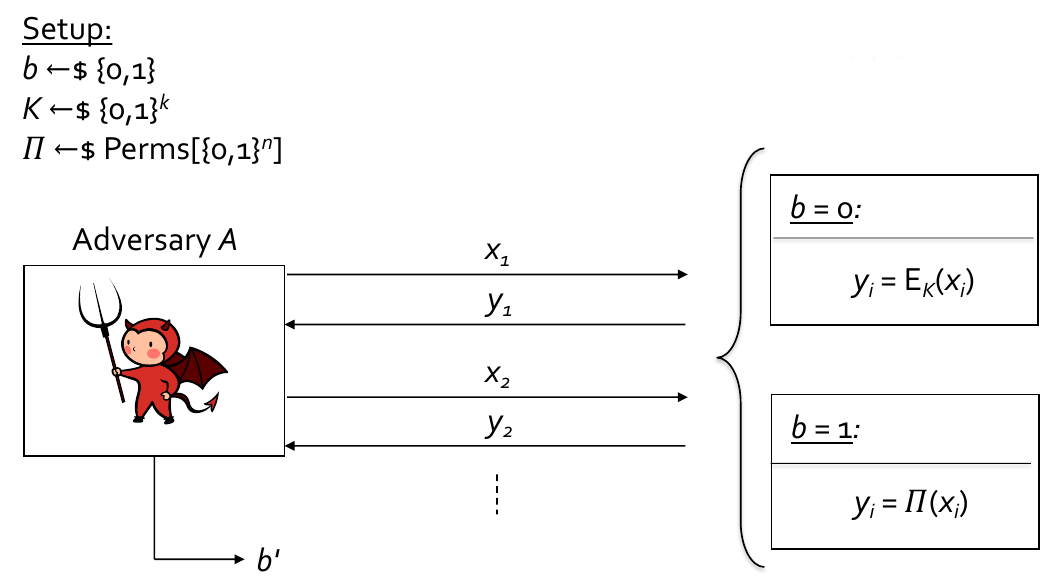
\includegraphics[scale=0.4]{images/prp.png}
    \caption{PRP game pictorially}
    \label{fig:prp}
\end{figure}

The advantage is defined as:
$$
\mathbf{Adv}^{PRP}_E (\A)
= 2 \cdot \Big| \Pr[ \text{Game}\textbf{PRP}(\A, E) \Rightarrow \text{true} ] - \frac{1}{2} \Big|
$$
where the probability is over the randomness of $b, K, \Pi, \A$.

\paragraph{Constructing block ciphers}
In general: keyed round function that is repeated many times.

\begin{itemize}
\item Feistel cipher: halved blocks crossing back and forth, e.g. DES
\item Substitution-permutation network: confusion + diffusion, e.g. AES
\end{itemize}


\subsection{Symmetric Encryption}


\subsection{Hash Functions}


\subsection{Message Authentication Codes MACs}


\subsection{Authenticated Encryption}

